\documentclass[12pt]{article}

% Language setting
% Replace `english' with e.g. `spanish' to change the document language
\usepackage[english]{babel}

% Set page size and margins
% Replace `letterpaper' with `a4paper' for UK/EU standard size
\usepackage[letterpaper,top=2cm,bottom=2cm,left=3cm,right=3cm,marginparwidth=1.75cm]{geometry}

% Useful packages
\usepackage{amsmath}
\usepackage{amsmath}
\usepackage{amssymb}
\usepackage{graphicx}
\usepackage[colorlinks=true, allcolors=blue]{hyperref}
\usepackage[11pt]{moresize}
\newcommand{\ts}{\textsuperscript}
\usepackage{enumitem}
\newcommand{\E}{\mathbb{E}}
\newcommand{\V}{\mathbb{V}}

\title{Multi-level Monte Carlo Methods}
\author{Aditya Ujeniya}
\date{November 14, 2022}

\begin{document}
\maketitle

\begin{abstract}
 At the state of art, a well-establish algorithm to compute expectation and high order moments of forward problem is Monte Carlo Method with computational complexity $\mathcal{O}(\epsilon\ts{-3})$. In several engineering applications, it is well established since 70s. Recently, an efficient version namely  Multilevel Monte Carlo allows to achieve better efficiency, exploiting the underlying hierarchy (multiscale) in space (and/or time) of numerical discretization, numerical solver (MultiGrid), and physical phenomena.  The fundamental idea of the algorithm is a variance reduction technique along the scales (levels) and expands the expectation by telescopic series. In the project, we describe the fundamental concepts and numerical experiment to study accuracy and efficiency. 
 
%Multilevel Monte Carlo is such a simple idea and it is more of an approach that can be applied to wide variety of applications. But each new application that we come to , there is some creativity involved in thinking through how to apply that. So, we will cover few application go through the report. We study Classic Monte Carlo method and while exploring classic technique for certain applications, we find that the total cost for Classic Monte Carlo is $ O(\epsilon\ts{-3}) $ in order to achieve Mean Squared Error of $ \epsilon $\ts{2}. Hence, we look at various techniques to reduce this huge cost and Multilevel Monte Carlo, amongst these cost reduction techniques, substantially reduces this total cost as compared to Classic method.
\end{abstract}

\section{Introduction}

The real world has lots of stochastic systems that we are pretty familiar with. By stochasticity we not only mean observation error but we also mean the noise or randomness. They are inherent part of dynamic systems. But sometimes we do not realize them. There are finance systems. They are heavily stochastic. A similar one we are pretty used to, last 2 years in particular, was the epidemics. They follow stochastic pattern as well. And then on another level, we know lots of cellular processes, particularly intracellular processes like gene expression. They have intrinsic stochasticity because these combinations of very small populations with certain biochemicals have big influence in dynamics. So, there's that randomness occurring at that level.



\section{Simulating Simple Stochastic Differential Equation}
Let us take a simple example from Computational Finance that requires solving Stochastic Differential Equations.
\subsection{Geometric Brownian Motion}
Geometric Brownian Motion (GBM) is a stochastic process over a continuous time interval where randomly varying motion - Brownian Motion or Wiener process with drift. Wiener process and drift term are explained below:

\clearpage
\begin{equation}
   d S_t = a(S_t, t) dt + b(S_t,t) dW_t   
\end{equation}

$a(S_t,t)$d$t$ is called Drift term which will be deterministic term \& $b(S_t,t)$d$W_t$ is the stochastic term with $b(S_t,t)$ as diffusion coefficient and d$W_t$ is the Wiener process or increment of Brownian Motion. Over a small time interval d$t$, this increment d$W_t$ is normally distributed and the variance is equal to d$t$. This is typically approximated by Euler Maruyama method.

\subsection{Euler Maruyama Method}
Euler Maruyama method corresponds to standard form of Euler time integration for Ordinary Differential Equation. 
\begin{equation}
\hat{S}({t}_{n+1}) = \hat{S}({t}_{n}) +a(\hat{S}({t}_{n}),t_n) \Delta T + b(\hat{S}({t}_{n}),t_n) \Delta  W_t 
\end{equation}
% i change a bit notation. meaning is the same.
We freeze drift term and diffusion term at the beginning of time step, treat them as constants. Then in simple finance applications, the quantity of interest is some function of the terminal value of this GBM Path '$S$' at a final time '$t$'. When we simulate a GBM Path, it looks something like this:

\begin{figure}[h!]
\centering
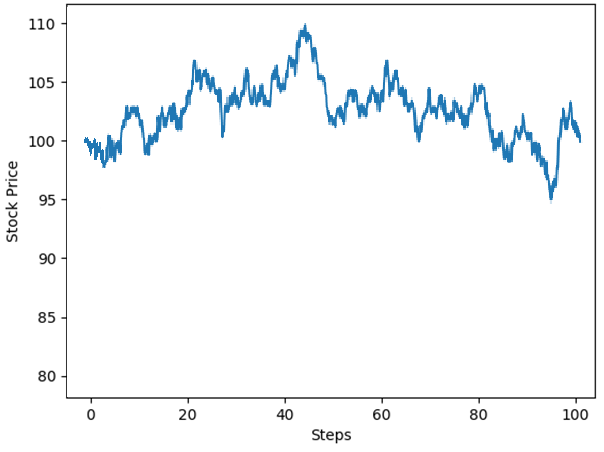
\includegraphics[width=0.6\textwidth]{GBE_Sim.png}
\caption{GBE Path Simulation using Euler Maruyama Method}
\end{figure}

Often, we are interested in estimating some averaged behavior. But since we do not have access to the probability density function, we use repeated simulations. And the technique of repeated simulations of stochastic processes is called Monte Carlo Simulation.
 
\clearpage

\section{Monte Carlo for GBE}
After simulating GBM using Monte Carlo, it looks something like this:
\begin{figure}[h!]
\centering
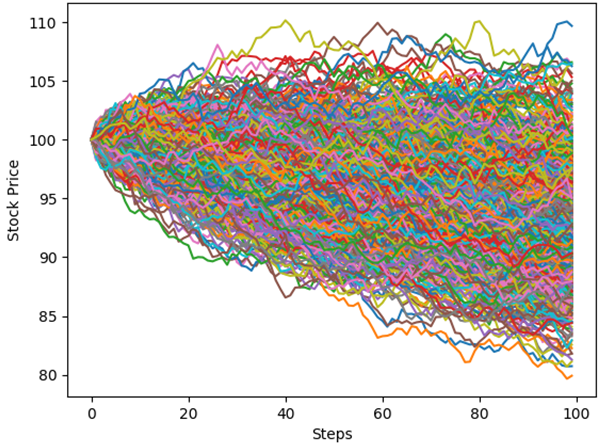
\includegraphics[width=0.6\textwidth]{GBE_MC_Sim.png}
\caption{Monte Carlo Simulation for our GBE Path Simulation}
\end{figure}

We have lots of simulation and we start to see more of a distribution forming. So this gives us an intuition of how we can use simulations to draw samples from this distribution and then we can approximate expectation using the average function value of all these realizations. To gain the expected behavior, we estimate the expectation using realizations $\hat{S}^1_t, \hat{S}^2_t, \ldots , \hat{S}^n_t$.
\begin{equation}
\E [\hat{S}_t] \approx \hat{P} = \frac{1}{N}\sum_{n=1}^{N} \hat{S}^n_t
\end{equation}

This is just a normal average, but it shares some interesting properties  with the  expectations that we are interested in. Because, even though $\hat{P}$ is a random variable, as $N \to \infty$, we know that $\hat{P}$ goes to true expectation. This is the expectation that we are interested in. Also, the variance $\V[\hat{P}] = \frac{\V[\hat{S}_t]}{N}$  shrinks proportional to $N$. Now depending on the variance of our system and how accurately we want to estimate in terms of precision, we could need a very large value of $N$. 

\subsection{Computational Challenge for GBE}

Now we would want to know the difference in error of true value and the expected value that we have calculated. The best way to quantify such errors is using Mean Squared Error (MSE). 

\begin{equation}
 \E[ ( \hat{P} - \E[\hat{S}_t] )^2 ] = \frac{\text{V}[\hat{P}]}{N} +  ( \E[\hat{P}] - \E[\hat{S}_t] )^2 \approx \frac{a}{N} + bk^2 
\end{equation}
 

MSE decomposes into bias which is the difference between true value and the calculated expected value. And we have the variance of the estimator which is coming from the fact that Monte Carlo is a random process. Now roughly or informally, we have approximate notation here, bias $\propto \epsilon$. We shrink bias, we shrink $\epsilon$. The bias is proportional to time step d$t$ in GBM. So it gets $k^2$ here.Variance is $\propto \frac{1}{N}$. We increase N, the number of simulations, we decrease variance. The variance term scales over the number of path calculations we perform. So, if we want to achieve Root Mean Squared Error (RMSE) of $\epsilon$, we nned MSE of $\epsilon^2$ and the number of path simulations (N) needs to scale like $\epsilon^{-2}$. But the size of time steps should scale like $\epsilon$. And the total computational cost will be $\frac{N}{k} = \epsilon^{-3}$. To improve the cost, we need:

\begin{enumerate}[label=\alph*]
\item Reduce N - variance reduction or Quasi Monte Carlo Methods.
\item Reduce the cost of each Path Simulation (on average) - MLMC.
\end{enumerate}

To reduce N, the number of independent samples that we take, there are lots of classic techniques in variance reduction which will leave total cost still as being $\epsilon^{-2}$, but they remove the multiplicative constant out front. Or we can use Quasi Monte Carlo methods $\Rightarrow$ rather than truly random numbers being generated, they are being constructed in a very systematic way that provides a better uniform coverage of probability space and the consequence of that is the total cost can be reduced, in best case, to $\epsilon^{-1}$. So those are classical methods in Monte Carlo literature.

But what we are going to do here with Multilevel is really tackle in reducing the cost of each our our Path Simulations. And let us see how we are going to do that.

\section{Two-level Monte Carlo}
Suppose there is some quantity that we want to estimate the expected value of i.e. 
$\E[\hat{P}_1]$. But there is some other quantity $\hat{P}_0$ which is much easier to simulate than $\hat{P}_1$ and $\hat{P}_0 \approx \hat{P}_1$ in some sense, then we have this trivial identity : 

\begin{equation} \E[\hat{P}_1] = \E[\hat{P}_0] + \E[\hat{P}_1 - \hat{P}_0]\end{equation} 

Rather than directly estimating the quantity on the left hand side, we are going to estimate each of the 2 quantities on the right hand side. 

\begin{equation} \frac{1}{N_0}\sum_{n=1}^{N_0} \hat{P}^n_0 + \frac{1}{N_1}\sum_{n=1}^{N_1} \hat{P}^n_1 - \hat{P}^n_0\end{equation} 

So we can estimate estimate standard Monte Carlo using $N_0$ samples and then the other one, we are going to estimate standard Monte Carlo but with different number of samples $N_1$. Now the point here is this $N_0$ is going to be roughly the same number of samples we could have used to estimate $\E[\hat{P}_1]$. But each of the $\hat{P}_0$ calculations are cheap compared to calculating $\hat{P}_1$. So the cost of calculating there is much less than corresponding calculations would have been for $\hat{P}_1$. And then the term $\hat{P}_1 - \hat{P}_0$, because $\hat{P}_0$ is close to $\hat{P}_1$ in some sense, the variance of the difference would also be a small value. Then because the variance is small, we need relatively few samples $N_1$ in order to accurately estimate the expected value. And that's where the saving are coming from. We are going to do relatively accurate calculations $\Rightarrow \hat{P}_1$ and will do lots of $\hat{P}_0 \Rightarrow$ but they are nice and cheap. Therefore, overall we save very substantially. Now as soon as we have 2 level approach like this, we can go to generalization with the whole sequence of levels.  

\clearpage

\section{Multilevel Monte Carlo}

Natural generalization gives us a sequence : $\hat{P}_0, \hat{P}_1, \ldots , \hat{P}_L$. 

\begin{equation} \E[\hat{P}_L] = \E[\hat{P}_0] + \sum_{l=1}^{L} \E[\hat{P}_l - \hat{P}_{l-1}]\end{equation} 

All the way from $\hat{P}_0$ to $\hat{P}_L$, $\hat{P}_L$ is going to be finest level of resolution and that's the one we want to get the expected value. For that, we have this decomposition of $\E[\hat{P}_0]$ and the telescopic sum of corrections. 

\begin{equation} \frac{1}{N_0}\sum_{n=1}^{N_0} \hat{P}^n_0 +  \sum_{l=1}^{L} \frac{1}{N_l} \sum_{n=1}^{N_l} \hat{P}^n_l - \hat{P}^n_{l-1}\end{equation} 

So we have the estimate for the first term and then the sum of estimates for the expected correction on each level.

\begin{figure}[h!]
\centering
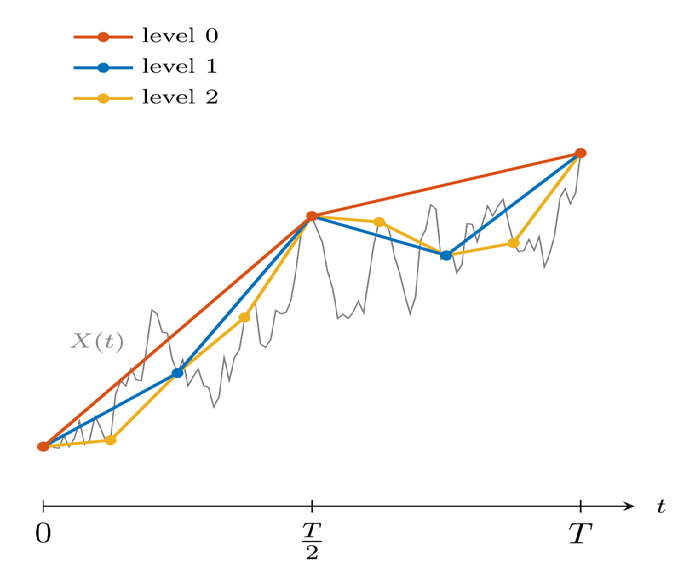
\includegraphics[width=0.6\textwidth]{MLMC_GBM.png}
\caption{Multi Level Monte Carlo Simulation for our GBM Path Simulation}
\end{figure}

In the given example we see that level 0 has less samples is highly biased approximation of the main GBM Path simulation. Next we increase more samples per level as we increase the number of levels. So the last level represents the accuracy of our estimate. It all depends on the last level $\Rightarrow$ how closely it approximates the true GBM Path such that the MSE between last level and the true GBM Path is less. Further, we are also going to see how to choose the number of levels optimally and how the number of samples per level have an effect in achieving certain MSE accuracy. 

\clearpage

\subsection{Reason for variance reduction in MLMC}

Each path simulation on different level will be a different random variable. So obviously the variance of each of these random variables will contribute to the total variance of the true Simulation. It should have made the problem worse by individual variance contribution from each level and then independent sum of these variance would make our problem worse. But there is a nice trick to it. The real reason why Multilevel Monte Carlo is useful because it induces positive correlation between $\hat{P}_l - \hat{P}_{l-1}$ Paths. In terms of correlated random variables, we get 

\begin{equation} \V[X-Y] = \V[X] + \V[Y] - C[X,Y]\end{equation} 

and if $C[X,Y]$ is positive, then this gives us variance reduction in whatever bias estimator we are going to do here. Now when we get reduction in variance, we need smaller samples for the expensive level L.

\subsection{How to choose samples on different levels}

Usually the samples per level $\tau_l $ is $ \propto m^{-l}$. It is demonstrated below in the image with an example.

\begin{figure}[h!]
\centering
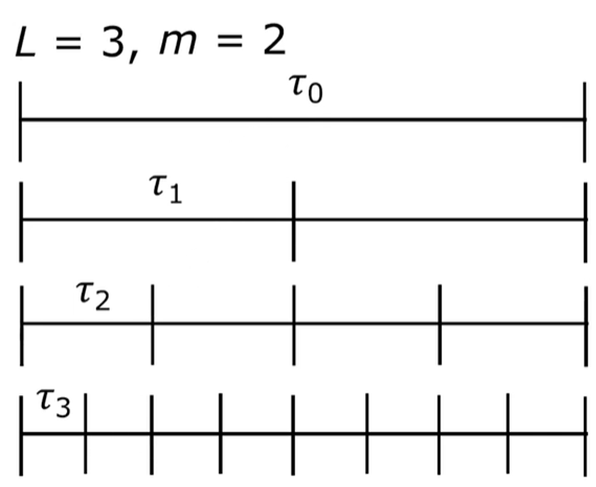
\includegraphics[width=0.6\textwidth]{Samples.png}
\caption{Number of levels and samples per level example}
\end{figure}

Since, in the example, m = 2, the samples per level will double the samples on previous level. It is optimal choice and most of the application choose to pick the factor of sampling per level as m = 2. Further more, in our experiments, we have doubled the number of samples per level quadratically. Because of this, we see quadratic convergence in expectation as compared to standard Monte Carlo simulation convergence. Though the cost per level also increases quadratically, the variance and mean is also reduced quadratically. So is the effect of choosing the sampling rate per level.

\clearpage

\subsection{Variance Reduction and Optimal Sample Size}

If we define,
\begin{itemize}
\item $C_0,\V_0$ to be cost and variance of level $\hat{P}_0$
\item $C_l,\V_l$ to be cost and variance of level $\hat{P}_l -\hat{P}_{l-1}$
\end{itemize}

then the total cost of MLMC is:

\begin{equation} \sum_{l=0}^{L} N_lC_l \end{equation}

where $N_L \Rightarrow$ Number of samples and $C_L  \Rightarrow$ Cost per sample.\linebreak
And the total variance of MLMC is given as:

\begin{equation} \sum_{l=0}^{L} \frac{1}{N_l}\V_l \end{equation}

After constrained optimization using Lagrangian Multiplier, we get these relations on equalities. To target MSE of $\epsilon^2$, we can optimize choice of L and $N_l$ for $l = 0, 1, \ldots, L$.

\begin{itemize}
\item Choose $N_l \propto \sqrt[]{\frac{C_l}{\V_l}}$ so that total variance is $ < \frac{1}{2}\epsilon^2$
\item Choose $L$ such that $ ( \E[\hat{P}_L] - \E[P] )^2 < \frac{1}{2}\epsilon^2$
\end{itemize}


\subsection{Caution}
Since MLMC required closer approximation of the original function, we need to take care of two things, Discontinuous functions and sudden jumps in functions. We demonstrate the later one because it poses a problem for MLMC convergence. Lets us look at an example in Figure 5. The reconstruction denotes the approximation of the original function at different levels, detail represent the difference in previous level approximation and the current level approximation. The error represents the MSE between level approximation and true function value. 
\par As and when go through the different levels for reconstructing the actual function, then the approximation at that level should minimize the MSE as levels increase. But if we see in the given example, increasing levels does not decrease the MSE such that it would not approximate the actual function and hence expected value target would not be achievable. Sudden jumps in function can cause such problems. Similarly, discontinuity also poses the same problem. So if the details do not decay, then the MLMC does not yield convergence.

\clearpage 

\begin{figure}[h!]
\centering
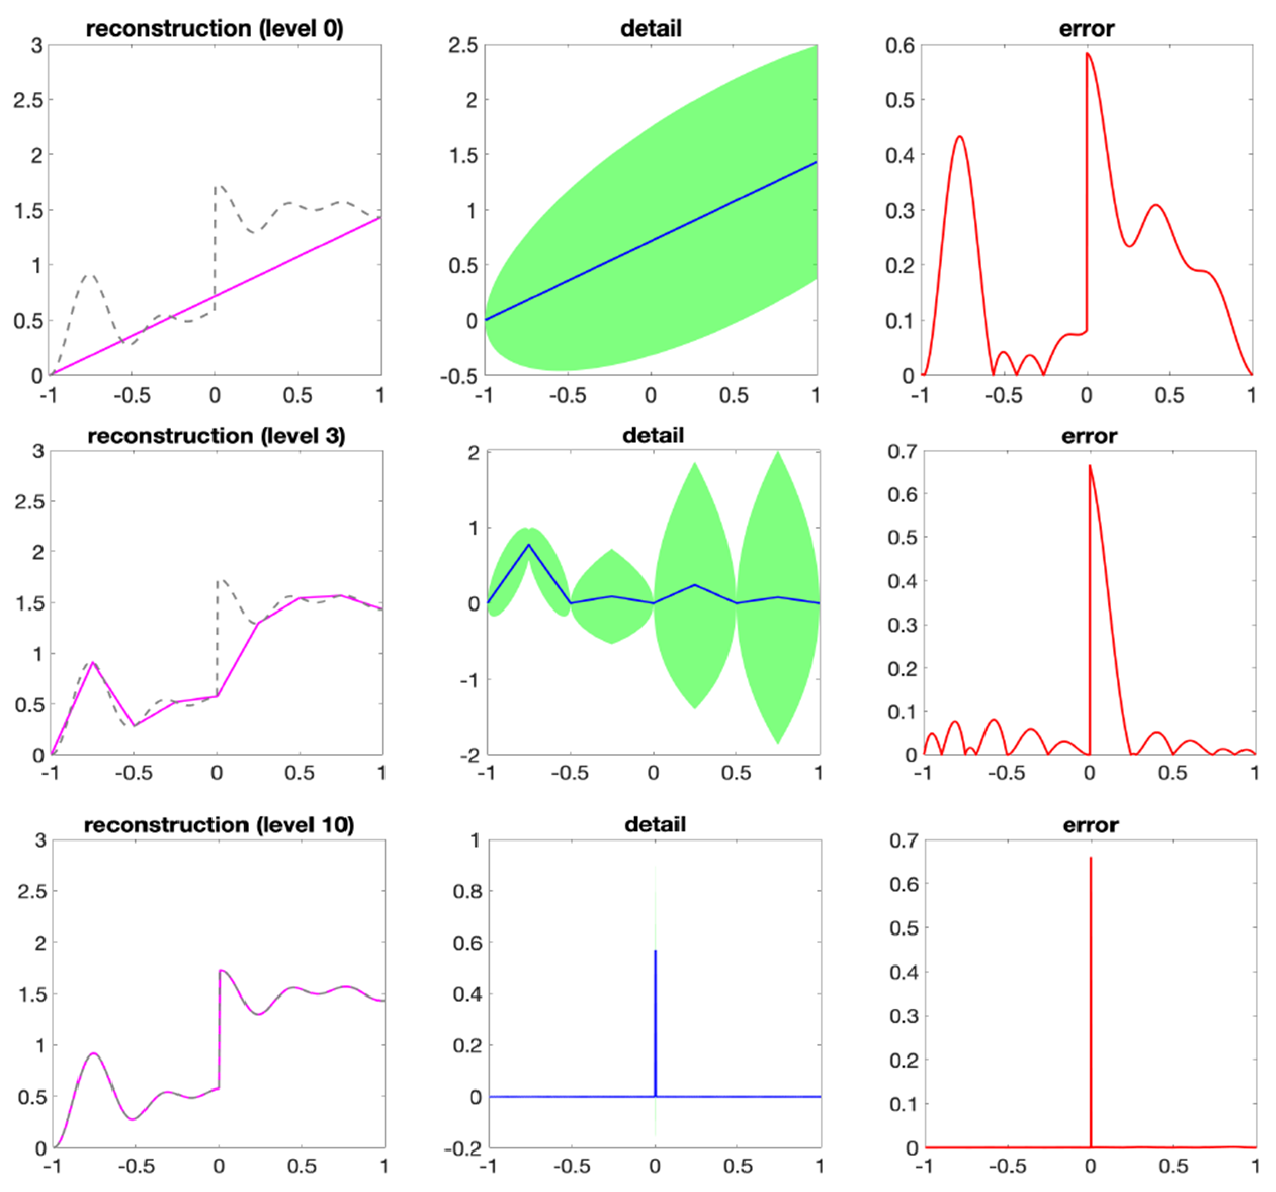
\includegraphics[width=0.8\textwidth]{CautionEx.png}
\caption{A highly jumping function at 0 with different level approximation and error between approximation.}
\end{figure}

\section{Results}
We ran some simulations for our Geometric Brownian Motion using Multi Level Monte Carlo method. Here we present the results for MSE  accuracy $\epsilon \in [ 0.005, 0.01, 0.02, 0.05, 0.1 ]$ with level min $L_{min} = 2 $ and level max $ L_{max} = 6$ for convergence check. 
\par 
To study these result tables, let us understand what the notation means:
\begin{itemize}
\item eps $\Rightarrow$ epsilon value/MSE accuracy.
\item value $\Rightarrow$ expected value.
\item $mlmc_{cost}$ $\Rightarrow$ MLMC total cost over all levels.
\item $std_{cost}$ $\Rightarrow$ Std. MC cost.
\item savings $\Rightarrow$ MLMC Cost Savings in terms of percentage compared to Std. MC.
\end{itemize}

\clearpage 

\begin{table}[h!]
\begin{center}
\caption{Table for cost of standard MC and MLMC}
\begin{tabular}{||c c c c c||} 
 \hline
 eps & value & $mlmc_{cost}$ & $std_{cost}$ & savings\\ [0.5ex] 
 \hline\hline
 5.000e-03 & 1.0451e+01 & 4.628e+07 & 2.949e+09 & 63.73\\ 
 \hline
 1.000e-02 & 1.0434e+01 & 8.429e+06 & 1.843e+08  & 21.87\\
 \hline
 2.000e-02 & 1.0442e+01 & 2.138e+06 & 4.608e+07 & 21.56\\
 \hline
 5.000e-02 & 1.0367e+01 & 2.412e+05 & 1.843e+06  & 7.64\\
 \hline
 1.000e-01 & 1.0458e+01 & 6.405e+04 & 4.608e+05 & 7.19\\ [1ex] 
 \hline
\end{tabular}
\end{center}
\end{table}

We see in Table 1 that as we go on increasing the accuracy, the total cost also goes on increasing. For $\epsilon = 0.005$, the difference in Std MC cost and MLMC cost is significant. It is 100x times less than Std. MC cost. We have enough percentage of savings at lower $\epsilon$. But if we go for less accuracy, i.e. $\epsilon = 0.01$, then the savings from MLMC are tangible and MLMC does not contribute much for simulation cost savings. Std. MC can do just fine with relatively few more samples than MLMC simulation. 

\begin{table}[h!]
\begin{center}
\caption{Table for number of samples for respective level}
\begin{tabular}{||c c c c c c||} 
 \hline
 eps & $N_0$ & $N_1$ & $N_2$ & $N_3$ & $N_4$\\ [0.5ex] 
 \hline\hline
 5.000e-03 & 19941517  & 1656286   & 406189  &  102404  &   26006\\ 
 \hline
 1.000e-02 & 4254591  &  353187    & 85705  &   21722 & \\
 \hline
 2.000e-02 & 1071060  &   90134    & 21902   &   5557 & \\
 \hline
 5.000e-02 & 147301   &  12191     & 2819 & &\\
 \hline
 1.000e-01 & 36247   &   2951     & 1000 & &\\ [1ex] 
 \hline
\end{tabular}
\end{center}
\end{table}
This Table 2 signifies the number of samples required at each level and the number of levels required to achieve the desired MSE accuracy. As we know, more deeper we go in terms of levels, more approximate would be the last level to the true function. Increasing MSE requires more accuracy, and hence we need more levels.

\begin{table}[h!]
\begin{center}
\caption{Table for details on different levels}
\begin{tabular}{||c c c c||} 
 \hline
 level & ave(Pf-Pc) & var(Pf-Pc) & cost per sample \\ [0.5ex] 
 \hline\hline
 0 &  1.0223e+01 & 1.618e+02 & 1.00e+00\\ 
 \hline
 1  &  2.0358e-01  & 4.458e+00  & 4.00e+00  \\
 \hline
 2 &  3.2319e-02 &  1.054e+00  & 1.60e+01  \\
 \hline
 3 & 7.1699e-03 & 2.736e-01 &  6.40e+01 \\
 \hline
 4 &  1.9255e-03 & 6.905e-02 & 2.56e+02\\
 \hline
 5 &  4.9564e-04 & 1.726e-02 &  1.02e+03 \\ [1ex] 
 \hline
\end{tabular}
\end{center}
\end{table}
Lastly, this Table 3 shoes us the details at each level. 
\begin{itemize}
\item ave(Pf-Pc) $\Rightarrow$ average between fine level and coarse level.
\item var(Pf-Pc) $\Rightarrow$ variance between fine level and coarse level.
\end{itemize}

For level 0, the average and the variance would be for level 0 simulation. From level 1, the average and variance would be between current level 1 and previous level 0 and so on. We can see variance decrease between levels as we go increasing the number of levels. Also, the average between levels show how the levels go on approximating the true function. As we go deeper with levels, they will highly approximate the true function and hence, the average and variance will reduce significantly between them. But approximating at deeper levels means more samples and the cost per sample will increase. Since we have set the number of samples to increase quadratically, the cost also increases quadratically as seen in the table.

\begin{figure}[h!]
\centering
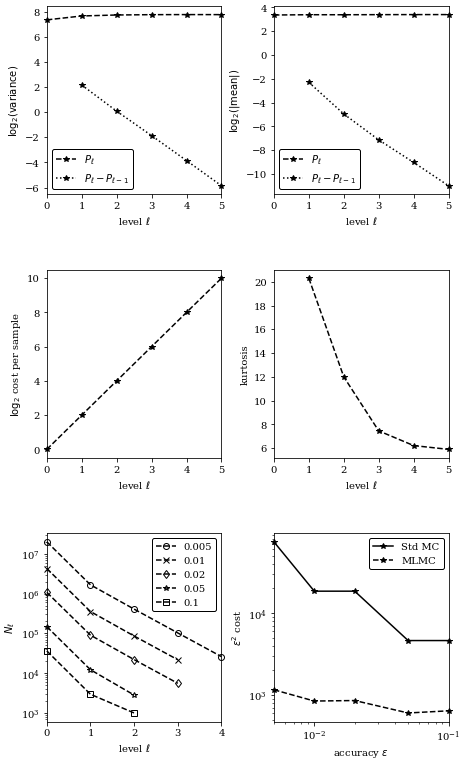
\includegraphics[width=0.6\textwidth]{opre_gbm1.png}
\caption{Plotting information from the tables.}
\end{figure}

Plotting the consolidated information from the constructed tables gives a nice sense on how the results look like altogether with all levels combined. If we take the variance and mean in $log_2$, the we can see linear decay between fine and coarse level. This is because we increase the number of samples per level quadratically, and extending this we see quadratic decrease in the graphs. Lastly, the comparison between Std. MC cost and MLMC cost gives significant insights. We discussed it previously that with higher accuracy, the savings with MLMC are of great importance than normal cost. Std. MC rises steeply as we increase the accuracy requirement.

\section{Applications and further extension}
There is lot of work done in optimising MLMC further than the basic idea as well as new application have found their way to implement MLMC and save the total simulation cost. We look at some examples and the extensions that have been carried out till now.
\subsection{Mixed Precision Computing}
As more examples of the flexibility of the MLMC approach, the levels can correspond to different levels of computing precision:
\begin{itemize}
\item 2l+2 bits of precision on level l when using Field Programmable Gate Arrays. This has been tried out by Korn, Ritter and Wehn in 2014.
\item IEEE half-precision on level 0, IEEE single precision on level1, etc., when computing on CPUs or GPUs. This way, since it computationally cheap to compute more half precision values and relatively fast to transfer them from memory to L1 cache, we can use MLMC this way and save more.
\end{itemize}

or the different levels can use different random number generators:
\begin{itemize}
\item level 0: 10-bit uniform random numbers, with table lookup to convert to approximate Normals.
\item level 1: 32-bit uniform random numbers, and more complex calculation to obtain Normals.
\end{itemize}

\subsection{Multi-index Monte Carlo}
Haji-Ali, Nobile and Tempone, in 2015, were able to extend MLMC along with combination technique to approximate stochastic models. In MIMC, they use higher order mixed difference instead of first order differences, to reduce the variance of the hierarchical finite differences in grids. We can think of MLMC as a Sparse Grid methods.

Standard "1D" MLMC truncates the telescopic sum as:
\begin{equation} \E[P] = \sum_{l=0}^{\infty}\E[\Delta\hat{P}_l] \end{equation}
where $\Delta\hat{P}_l = \hat{P}_l - \hat{P}_{l-1} $ and $\hat{P}_{-1} = 0 $
 
In "2D" MLMC truncates the telescopic sum as:
\begin{equation} \E[P] = \sum_{l1=0}^{\infty}\sum_{l2=0}^{\infty}\E[\Delta\hat{P}_{l1,l2}] \end{equation}
where $\Delta\hat{P}_{l1,l2} = (\hat{P}_{l1,l2} - \hat{P}_{l1-1,l2} )-(\hat{P}_{l1,l2-1} - \hat{P}_{ll-1,l2-1} )$

\section{Conclusion}
Multilevel idea is very simple idea.The key question is how to apply it in new situations, and how to carry out the numerical analysis. Discontinuous output functions can cause problems, but there is a lot of new techniques to cope up with it. It is being used for an increasingly wide range of applications and biggest computational savings when coarsest (reasonable) approximation is much cheaper than finest. Currently, using MLMC gets at least 100× savings for SPDEs and stochastic chemical reaction simulations.

% here bib file please use zotero.
% Reference put the articles
\section{References}
\begin{enumerate}[label=\alph*]
\item \url{https://www.youtube.com/watch?v=zK1ghzLbrgI}
\item \url{https://www.youtube.com/watch?v=PzrP6HGUAio}
\item \url{https://people.maths.ox.ac.uk/gilesm/files/OPRE_2008.pdf}
\item \url{https://en.wikipedia.org/wiki/Multilevel_Monte_Carlo_method}
\item \url{https://www.uni-kl.de/AG-Heinrich/papers/mmcm01.pdf}
\item \url{https://people.maths.ox.ac.uk/gilesm/files/acta15.pdf}
\item \url{https://eta.impa.br/dl/135.pdf}
\item \url{https://blogs.nvidia.com/blog/2019/11/15/whats-the-difference-between-single-double-multi-and-mixed-precision-computing/}
\item \url{https://arxiv.org/abs/1405.3757}
\end{enumerate}


\end{document}